\documentclass[11pt]{article}
\usepackage[T1]{fontenc}
\usepackage[utf8]{inputenc}
\usepackage{lmodern}
\usepackage[a4paper,margin=2.4cm,headheight=14pt]{geometry}
\usepackage{microtype}
\usepackage{amsmath,amssymb}
\usepackage{graphicx}
\usepackage{booktabs,tabularx,array,longtable}
\usepackage[font=small,labelfont=bf]{caption}
\usepackage{xcolor}
\usepackage{pdflscape}
\usepackage{float}
\usepackage{listings}
\usepackage{upquote}
\usepackage{fancyhdr}
\usepackage[numbers,sort&compress]{natbib}
\usepackage[colorlinks=true,linkcolor=blue!50!black,citecolor=blue!50!black,urlcolor=blue!50!black]{hyperref}
\usepackage{bookmark}

\graphicspath{{figures/}{../article/assets/}}
\newcommand{\HeldOut}{8,324}
\newcommand{\Common}{8,297}
\newcommand{\Positives}{314}
\newcommand{\Groups}{460}
\newcommand{\Excluded}{27}
\newcommand{\Draws}{2,000}
\newcommand{\TrainVariants}{19,409}
\newcommand{\TrainGroups}{1,127}
\newcommand{\ValVariants}{4,376}
\newcommand{\ValGroups}{282}
\newcommand{\ValPositives}{134}
\newcommand{\InnerVariants}{15,033}
\newcommand{\ControlsSeconds}{30.81}
\newcommand{\ControlsRSS}{278.1}
\newcommand{\PrevalenceTrain}{0.0379}
\newcommand{\TutVariants}{977}
\newcommand{\TutPositives}{44}
\newcommand{\TutGroups}{58}
\newcommand{\EnvPython}{3.11.16}
\newcommand{\EnvSklearn}{1.9.1}
\newcommand{\EnvNumpy}{1.26.4}
\newcommand{\OutputsZipShort}{6d1f0de2f359}

\makeatletter\let\inputtab\@@input\makeatother % expandable input for table bodies

\newcommand{\cfg}[1]{\texttt{#1}}
% Observed difference with 95% interval; \stackedci switches to a two-line cell for wide tables.
\newcommand{\ci}[3]{#1 [#2, #3]}
\newcommand{\stackedci}{\renewcommand{\ci}[3]{\begin{tabular}[t]{@{}l@{}}##1\\ {}[##2, ##3]\end{tabular}}}
% Allow URLs to break after any character (xurl is not installed).
\makeatletter
\g@addto@macro{\UrlBreaks}{\do\a\do\b\do\c\do\d\do\e\do\f\do\g\do\h\do\i\do\j\do\k\do\l\do\m\do\n\do\o\do\p\do\q\do\r\do\s\do\t\do\u\do\v\do\w\do\x\do\y\do\z\do\A\do\B\do\C\do\D\do\E\do\F\do\G\do\H\do\I\do\J\do\K\do\L\do\M\do\N\do\O\do\P\do\Q\do\R\do\S\do\T\do\U\do\V\do\W\do\X\do\Y\do\Z\do\0\do\1\do\2\do\3\do\4\do\5\do\6\do\7\do\8\do\9}
\makeatother
\renewcommand{\bibfont}{\small\raggedright}
\newcommand{\pk}[1]{P@#1}
\newcolumntype{L}{>{\raggedright\arraybackslash}X}
\renewcommand{\arraystretch}{1.12}
\setlength{\emergencystretch}{2em}
\urlstyle{same}

\lstset{basicstyle=\ttfamily\footnotesize,columns=fullflexible,keepspaces=true,breaklines=true,
  frame=single,framerule=0.3pt,rulecolor=\color{black!40},xleftmargin=2pt,xrightmargin=2pt,
  showstringspaces=false,upquote=true}

\pagestyle{fancy}
\fancyhf{}
\fancyhead[L]{\footnotesize Splicing scores for a fixed minigene budget}
\fancyhead[R]{\footnotesize Historical results; independent reproduction pending}
\fancyfoot[C]{\footnotesize \thepage}
\renewcommand{\headrulewidth}{0.3pt}

\hypersetup{pdftitle={Choosing a splicing score for a fixed minigene budget: an exploratory comparison of a supervised baseline, SpliceAI and Pangolin on MFASS},
  pdfsubject={Manuscript reporting existing computational results; independent reproduction pending},
  pdfkeywords={splicing, MFASS, SpliceAI, Pangolin, precision at k, benchmark}}

% Supplement S1: embed the byte-identical original article in the PDF (pdfTeX primitives).
\immediate\pdfobj stream attr {/Type /EmbeddedFile /Subtype /text#2Fplain} file {../article/published-original.md}
\edef\origobj{\the\pdflastobj}
\immediate\pdfobj {<< /Type /Filespec /F (S1-published-original.md) /UF (S1-published-original.md) /Desc (Supplement S1: original published article, byte-identical copy) /EF << /F \origobj\space 0 R >> >>}
\edef\origspec{\the\pdflastobj}
\pdfnames {/EmbeddedFiles << /Names [(S1-published-original.md) \origspec\space 0 R] >>}

\begin{document}

\begin{center}
{\LARGE\bfseries Choosing a splicing score for a fixed minigene budget:\\[2pt]
an exploratory comparison of a supervised baseline,\\[2pt] SpliceAI and Pangolin on MFASS\par}
\vspace{0.8em}
{\large Study repository \texttt{rewire-bio/splicing-model-selection}\par}
{\small Author list to be confirmed by the study owner. Drafted with AI assistance; see Section~\ref{sec:disclosure}.\par}
\vspace{0.6em}
{\small Original analysis: 29--30 September 2026. Manuscript compiled from the archived results: October 2026.\par}
\end{center}

\vspace{0.4em}
\noindent\fbox{\begin{minipage}{\dimexpr\linewidth-2\fboxsep-2\fboxrule\relax}
\small\textbf{Status of this manuscript.} This is a manuscript reporting \emph{existing} computational
results. Every number comes from a companion run executed on 29--30 September 2026, from the published
annotation-matched study whose saved scores that run replays, or from the cited literature. Numbers were
extracted and formatted from the archived outputs; nothing was recomputed for this manuscript. A fresh,
independent reproduction is \textbf{pending}: the reproduction protocol in the repository
(\texttt{protocol.md}, draft v2, unapproved) incorporates corrections from an automated AI methods review of draft v1
and has not been executed. No result here carries a verified or approved status. All
intervals are exploratory and unadjusted, because the held-out outcomes had been inspected in earlier work.
\end{minipage}}

\begin{abstract}
\noindent A laboratory that can run a fixed number $k$ of minigene splicing assays needs a score that
places as many splice-disrupting variants as possible in its first $k$. We compared a supervised
gradient-boosted $k$-mer baseline trained on assay labels with two zero-shot splice specialists,
SpliceAI and Pangolin, each with masking off and on, on the held-out arm of the MFASS exon-recognition
assay. SpliceAI and Pangolin scores were not regenerated: they are a saved-score replay of published
per-variant predictions from an annotation-matched study (GRCh38, GENCODE~44 canonical transcripts). On the
\Common{} held-out variants that every configuration scored (\Positives{} disrupting, \Groups{} exon/gene
groups), the historical baseline \cfg{kmer\_cons} placed 61 disrupting variants in its first 100, and the
four specialist configurations placed 63 to 66. No difference at $k=100$ was established: every paired
95\% whole-group bootstrap interval for the precision difference includes zero (for unmasked Pangolin,
$+0.040$ [$-0.038$, $+0.120$]), and together the intervals allow about 7 fewer to 13 more disruptions per 100.
This is not equivalence. Against a validation-selected version of the baseline the point differences
shrink to between $+0.000$ and $+0.030$. Pangolin had higher whole-list average precision
($+0.102$ [$+0.061$, $+0.142$] for the unmasked configuration) and AUROC, and at a budget of 300, chosen
after the budget curve had been seen, both Pangolin intervals exclude zero. That is a lead to test, not a
finding. We also document a failure mode: 23 held-out variants have recorded alleles that are the complement
of GRCh38, consistent with an inverted hg19-to-hg38 mapping that is not author-confirmed. The endpoint is
exon recognition in a synthetic reporter, not patient splicing or pathogenicity.
\end{abstract}

\tableofcontents
\clearpage

%======================================================================
\section{Introduction}\label{sec:intro}

Massively parallel minigene assays let a laboratory measure the splicing effect of many single-nucleotide
variants (SNVs), but each construct still has a cost. A group with capacity for $k$ constructs, and a
candidate list much longer than $k$, has to rank the list. The quantity that matters for that decision is
not a calibrated probability or a classification threshold but the number of splice-disrupting variants
among the first $k$ ranked candidates: the precision at budget $k$ (\pk{k}).

Two kinds of score are available. A supervised model trained on labels from the same assay design can learn
the reporter's idiosyncrasies, but needs thousands of labels. Zero-shot splice specialists such as
SpliceAI~\citep{jaganathan2019spliceai} and Pangolin~\citep{zeng2022pangolin} need no assay labels, but read
the genome around the variant rather than the construct, and their outputs depend on annotation and masking
settings. Earlier benchmarks have shown that the optimal score threshold for these tools varies between
exons, regions and variant classes~\citep{smith2023benchmarking}, which is one reason to rank at a budget
rather than threshold a score.

This manuscript reports a comparison of these workflows on the MFASS assay~\citep{chong2019mfass} at fixed
budgets. Its contributions are:
(i) a \pk{k} comparison on one common scored population, with explicit tie ranges and paired whole-group
bootstrap intervals, against both a historical and a validation-selected supervised baseline;
(ii) a description of how the answer depends on the budget, with the post hoc budgets marked;
(iii) a documented assembly-orientation failure mode: variants a pipeline would have scored without warning if
allele checks were skipped;
and (iv) a runnable companion that, in the original run, regenerated every control score and metric from pinned public
inputs (independent reproduction is pending).

Two scope statements apply throughout. First, the comparison is between \emph{workflows}, not architectures:
inputs, training data, ensemble size, masking rules and score definitions all differ between the
configurations. Second, the held-out outcomes had been inspected in earlier work on this benchmark, so every
interval is exploratory and none is adjusted for multiple comparisons.

%======================================================================
\section{Background and related work}\label{sec:background}

\subsection{The MFASS assay}
MFASS~\citep{chong2019mfass} places each variant in a 170\,bp construct --- a natural exon under 100\,bp with
at least 40\,bp of upstream and 30\,bp of downstream intron --- inside a three-exon minigene reporter integrated
once per HEK293T cell. Sorting cells by fluorescence gives an exon inclusion index. A splice-disrupting variant
(SDV) lowers the index by at least 0.5 in an exon whose wild-type index is at least 0.5. Of 27,733 ExAC
variants, 1,050 (3.8\%) were disrupting, 83\% of them outside canonical splice sites~\citep{chong2019mfass}.
Figure~\ref{fig:mfass} reproduces a published schematic of the reporter.

\begin{figure}[t]
\centering
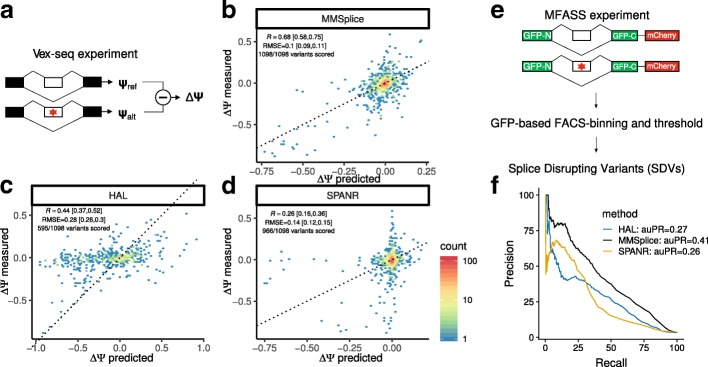
\includegraphics[width=0.92\linewidth]{14-chart-mmsplice-vexseq-mfass.jpg}
\caption{\textbf{The MFASS reporter and earlier predictors on it.} Panel~e shows the MFASS design: a split-GFP
minigene, sorting of cells into fluorescence bins, and the disruption threshold. Panels~a--d show a different
assay (Vex-seq). In panel~f each tool's precision--recall curve covers only the variants that tool could score,
so the subsets differ; SpliceAI and Pangolin are absent. Source: Cheng et al., \emph{Genome Biology} 2019,
Fig.~2~\citep{cheng2019mmsplice}, \url{https://pmc.ncbi.nlm.nih.gov/articles/PMC6396468/figure/Fig2/},
CC~BY~4.0, unmodified.}
\label{fig:mfass}
\end{figure}

\subsection{Splice specialists, masking and annotation}
SpliceAI~\citep{jaganathan2019spliceai,spliceai_repo} and Pangolin~\citep{zeng2022pangolin,pangolin_repo}
predict splice-site usage from sequence and report variant scores relative to annotated genes. Both offer a
``mask'' option, but equal flags are not equal operations: SpliceAI masks against the nearest annotated
boundary and Pangolin against every annotated site in the window. The defaults also differ: SpliceAI's
\texttt{-M} is 0, Pangolin's \texttt{-m} is True. A result reported for ``SpliceAI'' or ``Pangolin'' without these
settings does not identify what was run. Smith and Kitzman~\citep{smith2023benchmarking} showed that masking
and annotation choices change the set of variants each tool calls (Figure~\ref{fig:mask}).

\begin{figure}[t]
\centering
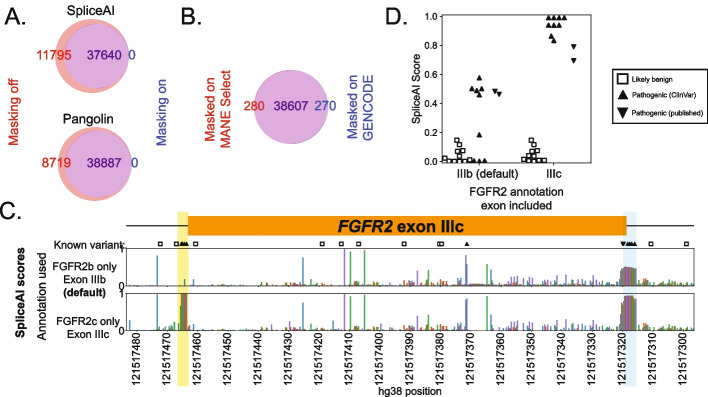
\includegraphics[width=0.92\linewidth]{13-chart-masking-and-annotation-effects.jpg}
\caption{\textbf{Masking and annotation change specialist calls.} Among 500,000 background variants, turning
masking on removed 11,795 SpliceAI calls and 8,719 Pangolin calls (panel~A; counts read from the figure).
Switching Pangolin between MANE Select and GENCODE annotation left 280 and 270 calls unique to each (panel~B).
Panels~C and~D show an FGFR2 exon whose scores depend on the annotated isoform. These are background calls,
not MFASS accuracy. Source: Smith and Kitzman, \emph{Genome Biology} 2023,
Fig.~6~\citep{smith2023benchmarking}, \url{https://pmc.ncbi.nlm.nih.gov/articles/PMC10734170/figure/Fig6/},
CC~BY~4.0, unmodified.}
\label{fig:mask}
\end{figure}

\subsection{Thresholds versus budgets}
Ranking at a budget avoids choosing a score threshold. In Smith and Kitzman's benchmark of eight predictors
on massively parallel splicing assays~\citep{smith2023benchmarking}, the best cut-off changed between exons,
regions and variant classes, and for SpliceAI, Pangolin and ConSpliceML was usually below the developers'
recommended value (0.2 for SpliceAI and Pangolin in that benchmark; Figure~\ref{fig:thresh}). The SpliceAI
cut-offs of $\geq 0.2$ and $\leq 0.1$ are ClinGen calibrations for clinical evidence~\citep{walker2023clingen},
not rules for filling an assay budget; 0.2 is also the SpliceAI authors' high-recall cut-off, and their README
calls 0.5 ``recommended''~\citep{spliceai_repo}.

\begin{figure}[t]
\centering
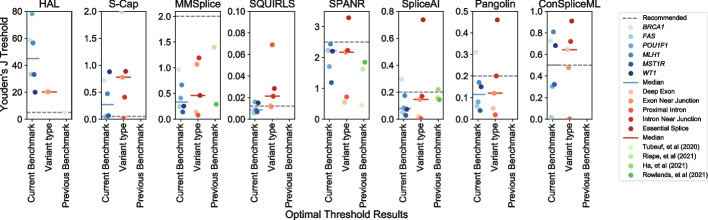
\includegraphics[width=0.95\linewidth]{12-chart-mpsa-threshold-variability.jpg}
\caption{\textbf{Optimal thresholds vary by dataset and variant type.} Youden-optimal thresholds for eight
predictors (points) by dataset, variant type and earlier report, against the benchmark's recommended threshold
(dashed line; 0.2 for SpliceAI and Pangolin). HAL and ConSpliceML optima span nearly the whole score range;
SpliceAI and Pangolin optima vary less and mostly fall below 0.2. None of the datasets is MFASS. Source: Smith
and Kitzman, \emph{Genome Biology} 2023, Fig.~5~\citep{smith2023benchmarking},
\url{https://pmc.ncbi.nlm.nih.gov/articles/PMC10734170/figure/Fig5/}, CC~BY~4.0, unmodified.}
\label{fig:thresh}
\end{figure}

\subsection{Other benchmarks}
MMSplice~\citep{cheng2019mmsplice} reported precision--recall curves on MFASS for MMSplice, HAL and SPANR, each
tool on the subset of variants it could score (Figure~\ref{fig:mfass}, panel~f); SpliceAI and Pangolin are absent
from that comparison. The CAGI5 splicing assessors~\citep{mount2019cagi5} caution that predicting a splicing assay
``cannot directly imply clinical significance'', a limit that applies equally here (Section~\ref{sec:limitations}).

%======================================================================
\section{Materials and methods}\label{sec:methods}

\subsection{Data and split}\label{sec:data}
The cohort was built by the companion's \texttt{build} step from the MFASS tables at the authors' repository,
commit \texttt{9a8e4f2}~\citep{kosurilab_mfass}. The build reads 32,669 source rows and keeps 27,733 eligible
variants (1,050 disrupting), matching the published counts; the paper's 2,198 exons are counted before the
eligibility filter, and the eligible variants span 2,185. Every eligible row passes an assay-pair check
(reference and mutant constructs differ only at the recorded position, with alleles consistent with strand).
The legacy \texttt{sequence} column is reverse-complemented in 7,770 rows, a detail that once led an earlier
baseline to centre its $k$-mer window on the wrong base~\citep{rb_mfass_readme}.

The split is the benchmark's canonical \texttt{split-v2}~\citep{rb_mfass_readme}: whole exon-and-gene groups
go to one arm, and no Ensembl gene identifier crosses arms. The training arm has \TrainVariants{} variants
(735 disrupting) in \TrainGroups{} groups; the held-out arm has \HeldOut{} variants (315 disrupting) in 463
groups. These build counts are reported as article text from the original run; the build log is not part of
the archived outputs.

\subsection{Common scored population and exclusions}\label{sec:population}
All four specialist configurations scored the same \Common{} of the \HeldOut{} held-out variants
(\Positives{} disrupting, \Groups{} groups). Every metric uses this common population; the \Excluded{}
unscored variants are excluded, not scored as negatives. One excluded variant is a disruptor. The
exclusions addendum of the benchmark~\citep{rb_exclusions} gives two causes:
\begin{itemize}
\item \textbf{23 assembly-orientation exclusions.} The recorded alleles are the complement of the GRCh38 base,
consistent with an inverted hg19-to-hg38 mapping whose strand and alleles were not converted. Both tools
refused these variants. The addendum traces 23 held-out records (21 from one CYFIP1 exon) and 90 cohort
records to this cause; 67 are in the training arm. Another AI coding agent (Codex) checked the explanation
computationally and it was reported upstream~\citep{mfass_issue1}; the MFASS authors have not confirmed it.
\item \textbf{4 annotation-span exclusions.} Four ARHGEF3 variants fall outside the GENCODE~44 canonical
transcript span, a consequence of the frozen transcript choice, not faulty variants.
\end{itemize}

\subsection{Configurations}\label{sec:configs}
Table~\ref{tab:configs} lists the ten configurations. Three evidence types are distinguished:
\emph{computed or fitted here} (scores produced by the companion's \texttt{controls} step on the training arm);
\emph{saved-score replay} (published per-variant SpliceAI and Pangolin predictions from the annotation-matched
study~\citep{rb_matched_readme}, re-evaluated without rerunning either tool); and specialist inference, which
was \emph{not run} for this work.

\begin{table}[t]
\centering
\footnotesize
\caption{\textbf{Configurations compared.} ``Fitted'' means trained on the \TrainVariants{} training variants
(\TrainGroups{} groups) and scored locally by the companion \texttt{controls} command. ``Replay'' means
published per-variant predictions from the annotation-matched study~\citep{rb_matched_readme} at
\texttt{093fd1a}, re-evaluated here. Overlap between MFASS and the specialists' training data was not audited.}
\label{tab:configs}
\begin{tabularx}{\linewidth}{@{}l L L l l@{}}
\toprule
Name & What it is & Inputs & MFASS labels & Scores \\
\midrule
\cfg{prevalence} & Training prevalence (0.038) for every variant & None & One number & Computed \\
\cfg{distance} & Negative distance to the nearest exon--intron junction in the construct & Construct layout & No & Computed (fixed rule) \\
\cfg{kmer\_assay} & Gradient-boosted trees on 3-mer frequencies in a 21\,bp window, construct position and alleles; published settings & Construct sequence and layout & Yes & Fitted \\
\cfg{kmer\_cons} & \cfg{kmer\_assay} plus phyloP and phastCons; the historical MFASS-v2 baseline, published settings & As above plus conservation & Yes & Fitted \\
\cfg{kmer\_*\_selected} & As above, hyperparameters chosen on held-aside training groups & As above & Yes & Fitted \\
\cfg{S0} / \cfg{S1} & SpliceAI 1.3.1, 5 models, mask 0 / 1, distance 50 & GRCh38 position and alleles; GENCODE~44 canonical annotation & No fitting & Replay \\
\cfg{P0} / \cfg{P1} & Pangolin \texttt{5cf94b8} with a per-gene masking patch, 12 models, mask False / True, distance 50 & As for SpliceAI & No fitting & Replay \\
\bottomrule
\end{tabularx}
\end{table}

\subsection{Controls and supervised baselines}\label{sec:controls}
\cfg{prevalence} assigns the training prevalence (\PrevalenceTrain) to every variant and serves as a no-information
floor. \cfg{distance} scores each variant by the negative distance, in bases, to the nearest exon--intron
junction in the construct (0 is the base touching a junction); it is a fixed rule with no fitting.
The two $k$-mer models reproduce the published MFASS-v2 baseline features (following \texttt{run\_baseline.py}
in rewire-benchmarks, MIT licence): position of the variant relative to both junctions and the construct,
exon and intron lengths, region and allele indicators, 3-mer frequencies in a 21\,bp window of the
assay-oriented mutant sequence, and, for \cfg{kmer\_cons}, phyloP and mean phastCons scores. Both use
scikit-learn's histogram gradient-boosted classifier (300 iterations, L2 regularisation 1.0, seed 20260914)
with the published settings (learning rate 0.06, 31 leaves). The companion's refit of \cfg{kmer\_cons}
reproduces the published baseline predictions byte for byte (SHA-256
\texttt{2f3117c2\ldots23eb}).

A validation-selected variant of each $k$-mer model was also fitted. A grid over learning rate
$\{0.03, 0.06, 0.1\}$ and leaves $\{15, 31\}$ was evaluated by average precision on a 25\% group-held-out part
of the training arm (\ValVariants{} variants, \ValGroups{} groups, \ValPositives{} disrupting); the test arm is
never read. The grid preferred 15 leaves for both models and learning rate 0.1 for \cfg{kmer\_cons}
(Appendix Table~\ref{tab:valgrid}), so validation selection disagrees with the published settings. The
historical baseline remains the default reference for every contrast; the selected versions appear only as a
labelled sensitivity analysis. Selection used average precision, whereas the decision endpoint is \pk{100}.

\subsection{Specialist saved-score replay}\label{sec:replay}
The matched study~\citep{rb_matched_readme,rb_matched_report,rb_matched_manifest} built both tools' annotation
from one \texttt{Ensembl\_canonical} transcript per gene in the GENCODE~44 GTF~\citep{gencode44} (the companion's
\texttt{annotation} step finds 62,754 such transcripts), used a scoring distance of 50 and patched Pangolin to
give each gene its own score arrays before masking~\citep{pangolin_issue29}; \cfg{P0} and \cfg{P1} are therefore
not stock Pangolin. Its settings correspond to SpliceAI \texttt{-D 50 -M 0} or \texttt{-M 1} and Pangolin
\texttt{-d 50 -m False} or \texttt{-m True}. The companion downloads the study's per-variant predictions at
commit \texttt{093fd1a} and re-evaluates them; the replay reproduces the study's AP and AUROC for all four
conditions to $10^{-12}$ and its registered-order \pk{100} exactly. Matching the annotation does not isolate
architecture: padding, masking rules, training data, ensemble size and score definition still differ.

\subsection{Metrics}\label{sec:metrics}
Each construct costs about the same whatever its result, so the primary metric is precision at budget $k$:
the fraction of the first $k$ ranked variants that disrupt splicing. The cost modelled is a construct that
shows no defect; missed disruptors are not costed, although recall is recorded. A random 100 would hold
about 4 disruptors. SpliceAI and Pangolin report two-decimal scores, so ties at the cut-off are common and are
handled explicitly. Let $c$ be the $k$-th highest score, $A$ the set of variants scoring above $c$ and $T$ the
set tied at $c$, with $p_A, p_T$ disrupting variants and $n_A, n_T$ variants in each; $r = k - n_A$ tied slots
remain. Then
\begin{equation}
\mathbb{E}[\mathrm{P@}k] = \frac{p_A + r\,p_T/n_T}{k},\qquad
\min = \frac{p_A + \max(0,\, r-(n_T-p_T))}{k},\qquad
\max = \frac{p_A + \min(r,\, p_T)}{k},
\end{equation}
where the expectation is over a uniformly random order of the tied block (Appendix~\ref{app:code} lists the
companion function verbatim). Paired contrasts instead use the \emph{registered tie order}: the matched study's
fixed, label-independent permutation of the variants. Average precision (AP; non-interpolated,
scikit-learn~\citep{sklearn_ap}) and AUROC summarise the whole ranking, which matters when the budget is large
or open.

\subsection{Paired bootstrap and interval inventory}\label{sec:stats}
Intervals are 95\% percentile intervals from \Draws{} whole-group bootstrap resamples (seed 20260914) of the
\Groups{} exon/gene groups, computed on the candidate-minus-baseline difference. Because a resampled list is
longer or shorter than the original, each draw keeps the review \emph{fraction} $k/8{,}297$ of its list, rather
than exactly $k$ variants; the realised depth was 21--31 for a nominal 25, 83--126 for 100 and 250--378 for 300
(Appendix Table~\ref{tab:depths}). The observed difference uses exactly $k$. No draw was single-class.

In this manuscript ``no difference established'' means that a paired 95\% interval for the difference includes
zero. That is not equivalence: such an interval can also include differences large enough to matter. The
benchmark protocol's improvement rule (a \pk{100} gain of at least 0.05 with a paired lower bound strictly above
zero~\citep{rb_protocol}) applies only to a future, prospectively registered cohort and is not applied here
either way. Interval bounds within about 0.005 of zero are described as ``at or near zero''; the Monte Carlo
error of the bootstrap endpoints was not quantified.

The study reports 41 substantive intervals, none adjusted for multiplicity: 9 from the matched study, all between
specialists (\cfg{S1}$-$\cfg{S0}, \cfg{P1}$-$\cfg{P0} and \cfg{P0}$-$\cfg{S0} on \pk{100}, AP and AUROC); 20
distinct intervals from the companion run against \cfg{kmer\_cons} (four specialists $\times$ \pk{25}, \pk{100},
\pk{300}, AP and AUROC; AP and AUROC repeat identically at each budget); and 12 against
\cfg{kmer\_cons\_selected}. The 12 tutorial-subset intervals in Appendix Table~\ref{tab:tutorial} are a pipeline check
and are neither counted nor interpreted.

\subsection{Pre-specified and post hoc analyses}\label{sec:posthoc}
Only $k=100$ was fixed in advance. Budgets 25 and 300 were chosen after the budget curve
(Figure~\ref{fig:budget}) had been seen, and the tables mark them post hoc. The validation-selected baseline contrasts
come from a separate run executed after the analyses above. The junction-distance breakdown and the shortlist-overlap
counts are descriptive outputs that \texttt{evaluate} prints for every configuration; they were not pre-specified as
endpoints and carry no intervals.

\subsection{Scoring checks}\label{sec:qc}
The companion's \texttt{check-variant} command runs the checks that decide whether a variant can be scored on
GRCh38: (1) the assay pair; (2) the GRCh38 base against the recorded genomic reference allele; (3) the 170\,bp
assay reference window against GRCh38 on the recorded strand; and (4) the GENCODE~44 canonical transcript and
distance to the nearest canonical exon end. It prints the public GRCh38 base but never the cohort's alternate
allele, because the MFASS repository declares no licence. Three worked examples, recorded in the original run
(Appendix~\ref{app:checkvariant}), illustrate the outcomes:
\begin{itemize}
\item A DDX1 intronic variant (\texttt{ENSE00000712808\_003}) passes checks 1--3 with 0 mismatching bases, lies
1\,bp from a canonical exon end and tops the unmasked Pangolin shortlist (S0 and S1 1.0000; P0 and P1 0.9100;
outcome disrupting). Its outcome was known beforehand, so this is a worked example, not validation.
\item A CYFIP1 variant (\texttt{ENSE00001321140\_001}) fails check 2: the recorded alleles are the complement of
the GRCh38 base, the window has 135 mismatching bases on the recorded strand and 0 on the opposite strand. The
assay is intact; the mapping inverted the region. It is excluded, not repaired.
\item An ARHGEF3 variant (\texttt{ENSE00002361772\_001}) passes checks 1--3 but lies about 80\,kb beyond the
canonical transcript (ENST00000296315.8), although ten alternative transcripts cover it; it is unscored under
the canonical-transcript protocol.
\end{itemize}
These checks matter because the 23 orientation mismatches surfaced only because both tools refused them; a
pipeline that skipped the reference-allele check, or flipped mismatched alleles automatically, would have scored
them without warning. A mismatched base should not be complemented unless the mapping orientation and sequence context
have been validated.

\subsection{Execution and provenance}\label{sec:provenance}
Every companion command reported in the original article, other than one illustrative example marked as not
executed, was executed on 29 and 30 September 2026 by an AI coding agent (Claude) on an Apple M4
CPU (16\,GB, macOS 26.6.2, uv 0.8.2, Python \EnvPython, NumPy \EnvNumpy, scikit-learn \EnvSklearn). The
companion fetches 14 pinned files with SHA-256 checks: the MFASS tables (about 80\,MB) from the authors'
repository at \texttt{9a8e4f2} and the split and saved predictions (about 2\,MB) from rewire-benchmarks at
\texttt{093fd1a}. The final revision was rerun from the archive in an empty directory with a fresh uv cache and
fresh downloads: every command exited 0, the decision tables, shortlists, exclusion lists and control
predictions were byte-identical, \texttt{metrics.json} differed only in timing fields, and the test suite
reported 26 passed. Those statements are part of the historical record; they were not re-executed for this
manuscript. The tables below are formatted from the archived run outputs
(\texttt{downloads/splice-shortlist-outputs.zip}, SHA-256 prefix \texttt{\OutputsZipShort}); each archive member's
digest is checked before use. Every generated value that also appears in the original article (evidence-map items
T2--T6, C-POP, C-OVERLAP, F4 and M-STUDY) is cross-checked against it; the remaining values are formatted directly
from the digest-checked archive members (Appendix~\ref{app:provenance}).

%======================================================================
\section{Results}\label{sec:results}

\subsection{At a budget of 100, no specialist configuration was separated from the baseline}\label{sec:b100}
Table~\ref{tab:b100} summarises all configurations at $k=100$. The historical baseline \cfg{kmer\_cons}
reached \pk{100} 0.610, the four specialist configurations 0.630 to 0.657, and the validation-selected baseline
0.630, the same point estimate as unmasked SpliceAI. The \cfg{distance} rule's 0.135 is an expectation over a
large tie: 171 variants share its top score (23 disrupting), so its first 100 can hold 0 to 23 disruptors.

\begin{table}[t]
\centering
\footnotesize
\setlength{\tabcolsep}{4pt}
\caption{\textbf{Budget 100 on the common \Common{} variants (\Positives{} disrupting, \Groups{} groups).} \pk{100}
is the expected value over random orders of the tied block, with the worst and best cases in brackets; ``Reg.''
is \pk{100} under the registered tie order; ``Scored'' counts variants scored of the \HeldOut{} held out; ``Tied'' is the number of variants tied at the cut-off score.
Recall is the expected recall at 100. Source: archived \texttt{out/metrics.json}, \texttt{methods}.}
\label{tab:b100}
\setlength{\tabcolsep}{3pt}
\begin{tabular}{@{}l l r l r r r r r@{}}
\toprule
Configuration & Scores & Scored & \pk{100} [tie range] & Reg. & Tied & Recall & AP & AUROC \\
\midrule
\inputtab{generated/tab_b100.tex}
\bottomrule
\end{tabular}
\end{table}

Table~\ref{tab:contrasts-hist} gives the paired differences against \cfg{kmer\_cons}. At 100, no \pk{100}
difference interval excludes zero; together they run from $-0.069$ to $+0.133$, which includes both a meaningful
loss and a meaningful gain. Under the least favourable tie order, \cfg{P1}'s $+0.050$ would be $+0.040$.

\begin{table}[t]
\centering
\footnotesize
\caption{\textbf{Paired differences against the historical baseline \cfg{kmer\_cons}.} Observed difference
(candidate $-$ \cfg{kmer\_cons}) with the 95\% whole-group bootstrap interval in brackets beneath it (\Draws{} draws,
seed 20260914, unadjusted, exploratory). \pk{k} differences use the registered tie order; at 300, tie order moves
\cfg{P0} by $-0.017$ to $+0.007$ and \cfg{P1} by $-0.007$ to $+0.010$. AP and AUROC do not depend on the budget.
Budgets 25 and 300 are post hoc. Each draw keeps the review fraction $k/8{,}297$ (realised depths in Appendix
Table~\ref{tab:depths}). Source: archived \texttt{out-b25/}, \texttt{out/} and \texttt{out-b300/metrics.json},
\texttt{paired\_contrasts}.}
\label{tab:contrasts-hist}
\stackedci
\setlength{\tabcolsep}{6pt}
\begin{tabular}{@{}l l l l l l@{}}
\toprule
Candidate & \pk{25} (post hoc) & \pk{100} & \pk{300} (post hoc) & AP & AUROC \\
\midrule
\inputtab{generated/tab_contrasts_hist.tex}
\bottomrule
\end{tabular}
\end{table}

\subsection{Whole-list metrics favour Pangolin (exploratory, unadjusted)}\label{sec:wholelist}
The whole-list metrics differ more than \pk{100}. Both Pangolin configurations have AP and AUROC intervals above
zero against the historical baseline (unmasked: AP $+0.102$ [$+0.061$, $+0.142$], AUROC $+0.099$ [$+0.073$,
$+0.125$]). Masked SpliceAI's AUROC interval against the historical baseline, $+0.037$ [$+0.005$, $+0.070$], excludes zero only
marginally (lower bound at or near zero; Monte Carlo error not quantified) among 41 unadjusted intervals, so it is not
read as an established difference.

\subsection{Sensitivity: the validation-selected baseline}\label{sec:selected}
The historical baseline is not the only defensible one. Table~\ref{tab:contrasts-sel} repeats the contrasts at
$k=100$ against \cfg{kmer\_cons\_selected} (learning rate 0.1, 15 leaves), from a separate run after the
analyses above with the same population, bootstrap and seed. The \pk{100} point differences shrink to between
$+0.000$ and $+0.030$ and every \pk{100} interval still includes zero; across both baselines about 9 fewer to 13
more disruptions per 100 remain possible. The Pangolin AP and AUROC intervals still exclude zero; masked
SpliceAI's AUROC interval again excludes zero only marginally (lower bound $+0.003$, at or near zero).

\begin{table}[t]
\centering
\footnotesize
\caption{\textbf{Paired differences against the validation-selected baseline \cfg{kmer\_cons\_selected} at
$k=100$.} Same population, bootstrap and seed as Table~\ref{tab:contrasts-hist} (realised depths 83--126); run after
the main analyses.
Source: archived \texttt{out-selected-b100/metrics.json}, \texttt{paired\_contrasts}.}
\label{tab:contrasts-sel}
\begin{tabular}{@{}l l l l@{}}
\toprule
Candidate & \pk{100} & AP & AUROC \\
\midrule
\inputtab{generated/tab_contrasts_sel.tex}
\bottomrule
\end{tabular}
\end{table}

\subsection{Specialist-versus-specialist contrasts}\label{sec:matched}
The matched study reported nine intervals, all between specialists (Table~\ref{tab:matched}). These values are
cited from that study, not recomputed by the companion. None of the three specialist contrasts established a
top-100 difference. The two masking contrasts have \pk{100} lower bounds of exactly 0.000 because \pk{100} moves in
steps of about 0.01 and many draws have a difference of exactly zero (22.5\% for SpliceAI masking, 44.4\% for
Pangolin masking). The \cfg{P1}$-$\cfg{P0} \pk{100} difference also depends on tie order: any label-independent
order gives \cfg{P1} 0.65 or 0.66. Masking raised AP within each tool without an established change in AUROC or
\pk{100}. Under matched annotation, unmasked Pangolin exceeded unmasked SpliceAI in AP and AUROC. No other
specialist pair was measured.

\begin{table}[t]
\centering
\footnotesize
\caption{\textbf{Specialist-pair contrasts reported by the annotation-matched study} (8,297 common variants, 314
disrupting, 460 groups; whole-group bootstrap, 2,000 draws, seed 20260914, 95\% percentile intervals; each draw keeps
the review fraction, realised depths 83--126). The
original article quoted five of these nine intervals; the remaining four (both masking \pk{100} upper bounds and
both masking AUROC intervals) and the \cfg{P1}$-$\cfg{P0} \pk{100} point value are transcribed from the study's
published README and contrast files at \texttt{093fd1a}~\citep{rb_matched_readme} without recomputation
(\texttt{evidence/paper-migration/matched-study-contrasts.json}).}
\label{tab:matched}
\begin{tabular}{@{}>{\raggedright\arraybackslash}p{4.4cm} l l l@{}}
\toprule
Contrast & \pk{100} & AP & AUROC \\
\midrule
\inputtab{generated/tab_matched.tex}
\bottomrule
\end{tabular}
\end{table}

\subsection{The answer depends on the budget}\label{sec:budget}
Figure~\ref{fig:budget} shows expected precision at the ten recorded budgets from 10 to 800 (values in Appendix
Table~\ref{tab:curve}). As fractions of this list, 25, 100 and 300 are 0.3\%, 1.2\% and 3.6\% of 8,297 variants,
against a prevalence of 3.8\%. The curves overlap from about 25 to 150; from about 200 the two Pangolin curves
are highest. SpliceAI is low at $k=10$ (0.548) because only three of its seven variants at score 1.00 are
disrupting. Table~\ref{tab:budgets} gives the tie ranges at the three tested budgets and
Figure~\ref{fig:forest} the paired differences.

\begin{figure}[t]
\centering
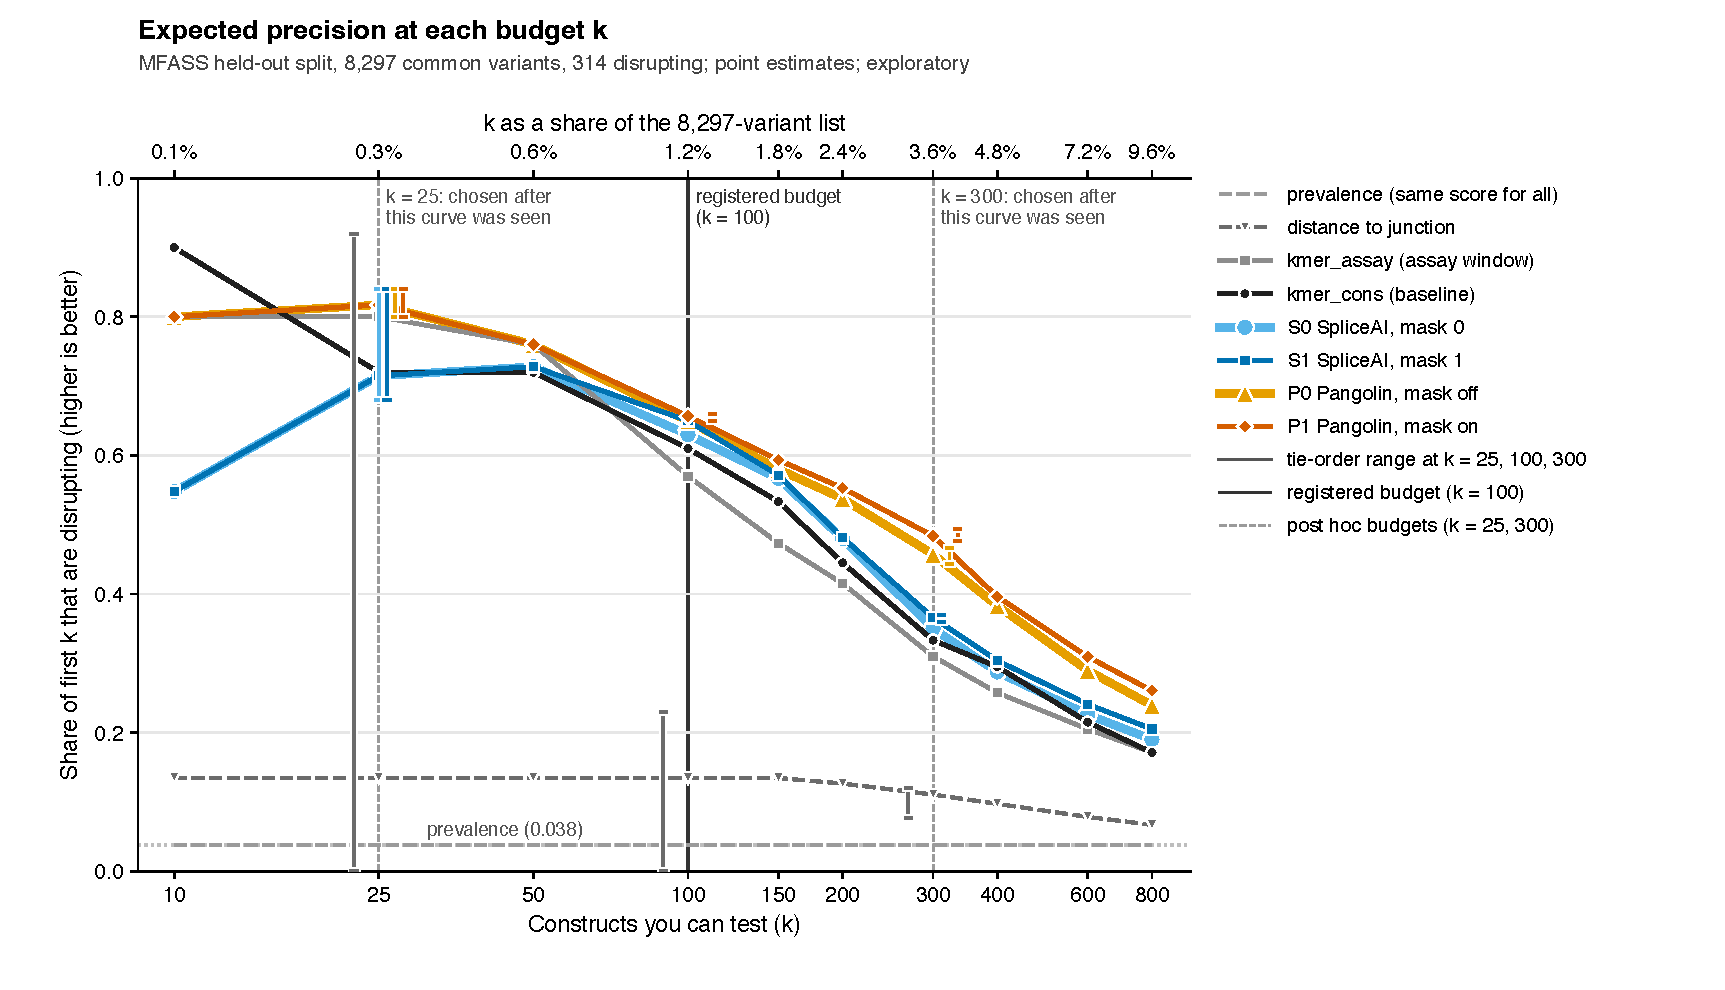
\includegraphics[width=\linewidth]{04-budget-curve.pdf}
\caption{\textbf{Expected precision at each budget $k$.} Lines show expected \pk{k} on the 8,297 common variants;
bars at 25, 100 and 300 are tie-order ranges. The tall grey bars belong to the \cfg{distance} rule (0.00 to 0.92
at 25); \cfg{prevalence} has no bar because every variant ties. Budgets 25 and 300 were chosen after this curve
had been seen. Source: original figure \texttt{article/assets/04-budget-curve.svg} (converted to PDF), drawn
from \texttt{out/metrics.json} \texttt{methods.<name>.budget\_curve} and the \texttt{precision\_at\_budget\_range}
fields of the three budget runs.}
\label{fig:budget}
\end{figure}

\begin{table}[t]
\centering
\footnotesize
\caption{\textbf{Expected precision at each tested budget with the range over tie orders} on the 8,297 common
variants. Point estimates only; paired intervals are in Table~\ref{tab:contrasts-hist}. Budgets 25 and 300 are
post hoc. Source: archived \texttt{methods} blocks of \texttt{out-b25/}, \texttt{out/} and
\texttt{out-b300/metrics.json} (identical to their \texttt{decision-table.md}).}
\label{tab:budgets}
\begin{tabular}{@{}l l l l@{}}
\toprule
Configuration & \pk{25} [tie range] & \pk{100} [tie range] & \pk{300} [tie range] \\
\midrule
\inputtab{generated/tab_budgets.tex}
\bottomrule
\end{tabular}
\end{table}

\paragraph{Budget 25 (post hoc).} The four measured difference intervals each span more than 0.4 and all include
zero (Table~\ref{tab:contrasts-hist}). No other pair was tested at 25, including the baseline against its
validation-selected version. Point estimates are fragile: \cfg{kmer\_cons} finds 18, \cfg{kmer\_assay} 20,
\cfg{kmer\_cons\_selected} 21, Pangolin 20 or 21 and SpliceAI 17 to 21. Hyperparameters alone move the baseline
from 0.720 to 0.840, more than any specialist point difference.

\paragraph{Budget 300 (post hoc).} Expected yields are about 100 for \cfg{kmer\_cons}, 105 and 110 for SpliceAI, and
137 (133 to 140 by tie order) and 145 (143 to 148) for \cfg{P0} and \cfg{P1}. The two Pangolin difference intervals
exclude zero, $+0.127$ [$+0.080$, $+0.172$] and $+0.150$ [$+0.099$, $+0.199$]; the SpliceAI intervals do not. These
are the only budget-based contrasts whose intervals exclude zero, and both rest on a post hoc budget. The
validation-selected baseline was not tested at 300.

\begin{figure}[t]
\centering
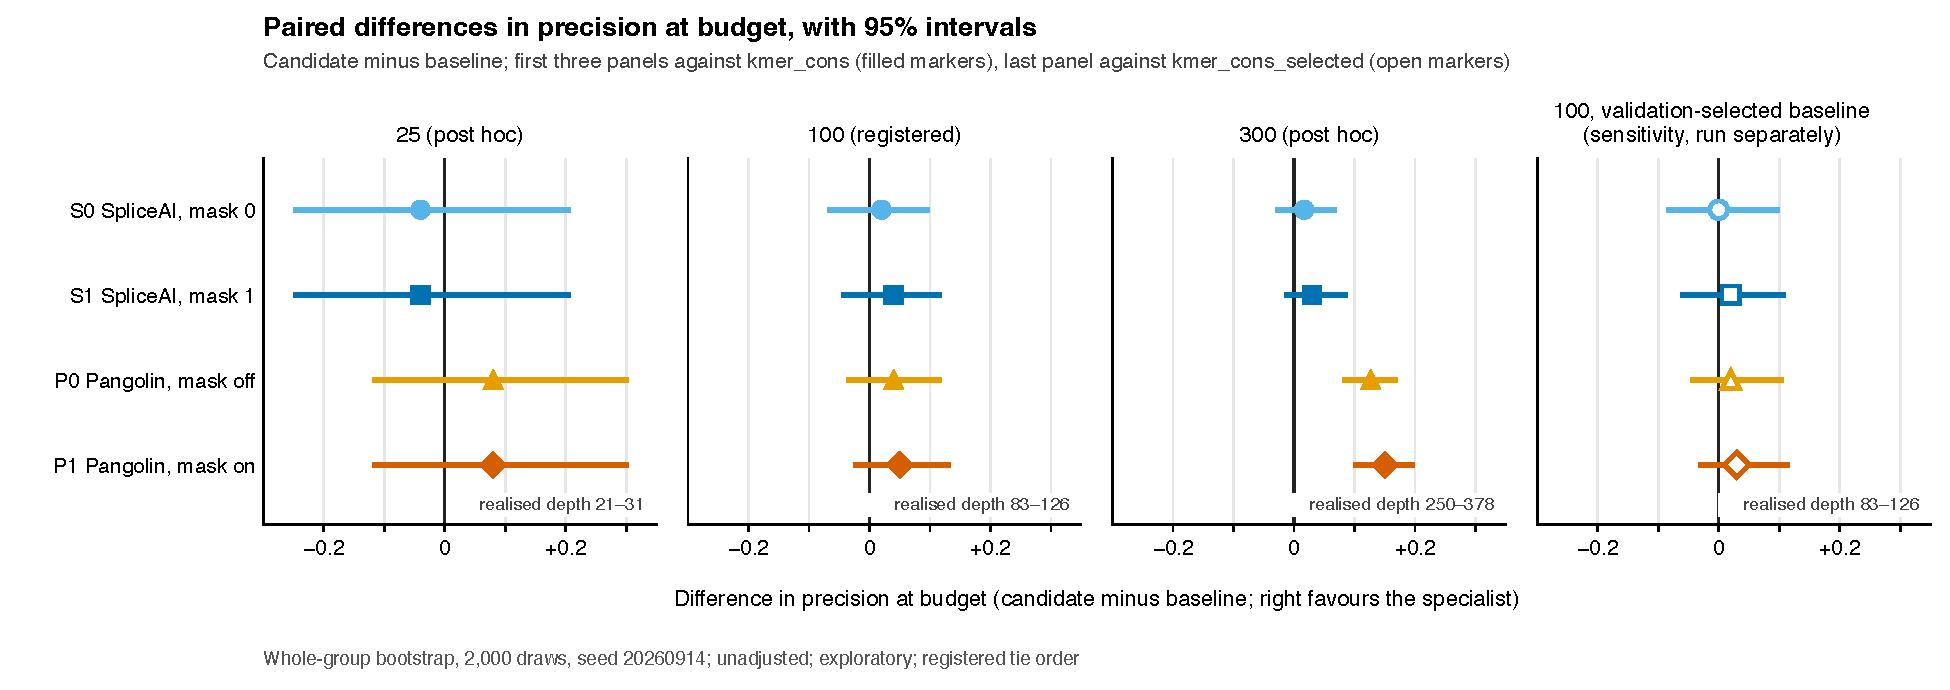
\includegraphics[width=\linewidth]{05-paired-differences-forest.pdf}
\caption{\textbf{Paired \pk{k} differences with 95\% whole-group bootstrap intervals.} Panels show
\cfg{S0}, \cfg{S1}, \cfg{P0} and \cfg{P1} minus the historical baseline at budgets 25, 100 and 300, and a separately
run panel at 100 against the validation-selected baseline. At 25 and 100 every interval includes zero (at 100,
against either baseline). At 300 (post hoc) both Pangolin intervals exclude zero. Source: original figure
\texttt{article/assets/05-paired-differences-forest.svg} (converted to PDF), drawn from the
\texttt{paired\_contrasts} of \texttt{out-b25/}, \texttt{out/}, \texttt{out-b300/} and \texttt{out-selected-b100/metrics.json}.}
\label{fig:forest}
\end{figure}

\subsection{Ties and shortlist composition}\label{sec:ties}
Ties are a separate problem from scoring checks. At $k=25$, both SpliceAI configurations have 7 variants at 1.00
(3 disrupting) and 23 tied at 0.99 (19 disrupting) for the remaining 18 slots, so the first 25 hold 17 to 21
disrupting variants (\pk{25} from 0.68 to 0.84). The registered tie order happened to give 17, which is why
SpliceAI's \pk{25} contrast in Table~\ref{tab:contrasts-hist} is $-0.040$. The exported budget-25 shortlist
therefore has 30 rows, 23 of them flagged as tied with the cut-off; its rank within a tied block is arbitrary. At
100, masked Pangolin has 3 variants tied at 0.54 for 2 slots, one disrupting, so its \pk{100} is 0.65 or 0.66.
A tie rule should be fixed before any outcome is seen, such as a seeded random permutation, or the whole tied
block should be tested.

Under the registered tie order, the first 100 of \cfg{kmer\_cons} and \cfg{P0} share only 61 variants, and \cfg{S0}
and \cfg{P0} share 88 (all pairs in Appendix Table~\ref{tab:overlap}). Two disrupting variants illustrate the
disagreement (reported in the original article from the companion run; their identifiers are not in the
archived outputs, so these values are imported and not independently re-checked). An IPO9 disrupting variant 3\,bp
from an exon end is ranked 1,092nd by \cfg{kmer\_cons} and 81st to 87th by the four specialists. A COL1A2 disrupting
variant, also 3\,bp from an exon end, is ranked 95th by \cfg{kmer\_cons}; unmasked SpliceAI scores it 0.00, one of
4,448 variants tied at ranks 3,850 to 8,297, and unmasked Pangolin 0.05, one of 182 tied across ranks 795 to 976.

\subsection{Where the disruptors are: junction-distance bands}\label{sec:bands}
Table~\ref{tab:bands} breaks the captured disruptors down by distance to the nearest exon--intron junction in
the construct. At 100, most captured disruptors lie within 10 bases of a junction (51 of 61 for \cfg{kmer\_cons},
57 of 65 for \cfg{P0}), and \cfg{kmer\_cons} captures slightly more at 11--30 bases (10 against 8). No top 100 reaches
the 30 disruptors beyond 30 bases, although 173 of the 314 lie more than 10 bases out. At 300, 36 of \cfg{P0}'s 38
extra disruptors over \cfg{kmer\_cons} (43 of 45 for \cfg{P1}) are 3 or more bases from a junction. Pangolin reaches 5
or 6 distant disruptors against none for the $k$-mer models: small counts at a post hoc budget. No band intervals
were computed. Appendix Table~\ref{tab:bands-full} gives every configuration at all three budgets.

\begin{table}[t]
\centering
\footnotesize
\setlength{\tabcolsep}{4pt}
\caption{\textbf{Disrupting variants captured in each top 100 and top 300} (registered tie order), by distance to
the nearest exon--intron junction in the 170\,bp construct (0 is the base touching a junction), with within-band
AUROC at the right. Descriptive, not pre-specified; the top-300 columns inherit the post hoc status of that budget; no
band intervals were computed. Source: archived
\texttt{out/metrics.json} and \texttt{out-b300/metrics.json}, \texttt{junction\_distance\_bands}.}
\label{tab:bands}
\begin{tabular}{@{}l r r r r r r r r c@{}}
\toprule
 & & & \multicolumn{3}{c}{Top 100} & \multicolumn{3}{c}{Top 300 (post hoc)} & AUROC in band \\
\cmidrule(lr){4-6}\cmidrule(lr){7-9}
Band (bases) & Variants & Disrupting & \cfg{kmer\_cons} & \cfg{P0} & \cfg{P1} & \cfg{kmer\_cons} & \cfg{P0} & \cfg{P1} & \cfg{kmer\_cons} / \cfg{P0} \\
\midrule
\inputtab{generated/tab_bands.tex}
\bottomrule
\end{tabular}
\end{table}

\subsection{Resources and coverage}\label{sec:resources}
The controls are cheap: loading, the 12-fit validation grid, final fits and scoring of 8,324 rows took
\ControlsSeconds\,s end to end with \ControlsRSS\,MB peak resident memory on the Apple M4 (the separate
\texttt{build} step peaks at about 680\,MB), and need only the MFASS tables (about 80\,MB), which include
conservation scores. The specialist times in Table~\ref{tab:resources} are the matched study's recorded times
for one sequential run on the same CPU type with 5 (TensorFlow) or 6 (Torch) threads, excluding cohort
preparation; peak memory was not recorded. The study recorded about 14\,h of wall time for the four conditions.
Running a specialist yourself requires about 1.13--1.14\,GB of downloads (Appendix Table~\ref{tab:downloads}). The
specialists scored 8,297 of 8,324 held-out variants; archived runs with other annotations scored 8,194 and 8,301
and are not pooled here~\citep{rb_matched_readme}.

\begin{table}[t]
\centering
\footnotesize
\caption{\textbf{Recorded compute.} Controls were measured in the companion run; specialist scoring times were
recorded by the matched study (\texttt{score\_test} covers 8,324 held-out rows). Peak memory for the specialists
was not recorded. Source: archived \texttt{out/metrics.json}, \texttt{resources}; \texttt{runs/controls/receipt.json}.}
\label{tab:resources}
\begin{tabularx}{\linewidth}{@{}L l l l@{}}
\toprule
Step & Evidence & Time & Peak memory \\
\midrule
\inputtab{generated/tab_resources.tex}
\bottomrule
\end{tabularx}
\end{table}

\subsection{Reproduction status}\label{sec:repro-status}
\noindent\fbox{\begin{minipage}{\dimexpr\linewidth-2\fboxsep-2\fboxrule\relax}\small
\textbf{Not yet reproduced under this repository's harness.} The values above are imported from the 2026-09-29/30
companion run. The repository's reproduction protocol (\texttt{protocol.md}, draft v2, unapproved) incorporates
corrections from an automated AI methods review of draft v1; draft v2 itself has not been reviewed, approved or
executed, and no reproduction outcome class is reported. When a run is approved and ends, its results are to be shown next to these imported values, including
any discrepancies, rather than replacing them.
\end{minipage}}

%======================================================================
\section{Discussion}\label{sec:discussion}

\subsection{What the evidence supports}
At the one pre-specified budget, roughly 1.2\% of this list, the specialists' point estimates were 2 to 5
disruptors per 100 higher than the historical supervised baseline and 0 to 3 higher than its validation-selected
version, but no difference was established and the intervals are wide enough to include a meaningful loss. Both
supervised baselines need same-design labels, and \cfg{kmer\_cons} also needs conservation tracks (it scored every
variant in about 30\,s with no genome download, but a new list needs both the tracks and thousands of labels);
\cfg{kmer\_assay} (\pk{100} 0.570) needs no conservation. The specialists need GRCh38 coordinates, allele and strand
checks and a canonical annotation. Choosing between them at this budget is therefore
reasonably made on cost, coverage and the availability of labels rather than on the measured precision.

Whole-list metrics tell a more consistent story for Pangolin: higher AP and AUROC than both baselines and than
unmasked SpliceAI under matched annotation, and, at the post hoc budget of 300, precision differences against the
historical baseline whose intervals exclude zero. Because 300 was chosen after the curve was seen and none of the
41 intervals is adjusted, this is a lead to test prospectively, not a finding.

\subsection{Decision guidance}
Table~\ref{tab:glance} summarises where to start, by label availability and budget fraction; Appendix
Figure~\ref{fig:flow} draws the same routes as a flowchart. Budgets are fractions of this one list: 8,297 MFASS
variants with 3.8\% prevalence and MFASS's short-exon case mix. A list with a different size, case mix or assay
needs its own labelled validation before these results guide the choice, so each row says where to start a pilot,
not where to set a threshold.

\begin{table}[t]
\centering
\scriptsize
\caption{\textbf{Where to start, by budget fraction and label availability} (MFASS-like minigene endpoint).
``Same-design labels'' are assay labels from the same construct design. Budgets are fractions of this list of
8,297 variants, not thresholds for other lists.}
\label{tab:glance}
\begin{tabularx}{\linewidth}{@{}>{\raggedright\arraybackslash}p{2.6cm} L L L@{}}
\toprule
Situation & Where to start & What the evidence shows & Main caveat \\
\midrule
Same-design labels; about 1.2\% of the list (tested at 100) & Either baseline or any specialist; choose on cost and coverage (Table~\ref{tab:b100}) & No \pk{100} interval excludes zero, against either baseline (Tables~\ref{tab:contrasts-hist}, \ref{tab:contrasts-sel}) & Not equivalence: about 9 fewer to 13 more disruptions per 100 remain possible \\
No assay labels; about 1.2\% (tested at 100) & A specialist, after GRCh38 allele, strand and transcript checks; choose on runtime, downloads and licence & \cfg{distance} finds about 13 per 100, the specialists 63 to 66 (Table~\ref{tab:b100}); no specialist-pair top-100 difference established (Table~\ref{tab:matched}) & \cfg{distance} versus specialists was not tested; \cfg{P0}$-$\cfg{S0} allows about 3 fewer to 8 more per 100 \\
Same-design labels; about 3.6\% (tested at 300, post hoc) & Pilot Pangolin (\cfg{P0} or \cfg{P1}) & Both Pangolin \pk{300} intervals exclude zero against the historical baseline (Tables~\ref{tab:contrasts-hist}, \ref{tab:bands}) & Post hoc budget; validation-selected baseline not tested at 300 \\
Same-design labels; about 0.3\% (tested at 25, post hoc) & Fix the tie rule before testing & No measured interval excludes zero (Table~\ref{tab:contrasts-hist}); ties move SpliceAI by up to 4 of 25 and hyperparameters move the baseline by 3 (Table~\ref{tab:budgets}) & Post hoc budget; point estimates are fragile \\
No labels at any fraction other than about 1.2\%; labels at any fraction other than about 0.3, 1.2 or 3.6\% & Pilot before committing; without labels, start with a specialist & Point estimates only (Figure~\ref{fig:budget}); without labels, \cfg{P0} had higher AP and AUROC than \cfg{S0} (exploratory) & No \pk{k} contrast was tested at these fractions \\
Every variant must be scored & Expect losses from coordinate and annotation mapping & Specialists scored 8,297 of 8,324 & Losses on another list depend on its mapping to GRCh38 and canonical transcripts \\
Patient RNA, pathogenicity or another reporter & None of these routes transfers & --- & Pilot a labelled subset in the target assay \\
\bottomrule
\end{tabularx}
\end{table}

\subsection{What would change these conclusions}
A prospectively registered comparison on an MFASS-like library with unseen outcomes, and with budget, tie rule,
comparator and candidate fixed in advance, would replace the exploratory status of every row. If a specialist met
the protocol's improvement rule~\citep{rb_protocol} there against a baseline trained on that library, it would
become the recommendation where labels exist. Without labels, the deciding contrast is Pangolin against SpliceAI,
tested the same way. If Pangolin's lead at about 3.6\% of the list did not reappear, the advice to pilot Pangolin
first at that fraction would be withdrawn. An author-confirmed liftover correction would return the 23 exclusions
and change the denominator. Patient RNA outcomes would answer a different question.

%======================================================================
\section{Limitations}\label{sec:limitations}
\begin{itemize}
\item \textbf{Exploratory status and budgets.} The held-out outcomes had been inspected before, so every interval is
exploratory and unadjusted for the 41 intervals reported. Only $k=100$ was set in advance; 25 and 300 are post hoc,
and the conclusion changes between 100 and 300. Every \pk{k} figure applies to this fixed population and case mix.
\item \textbf{Monte Carlo error.} The bootstrap endpoints' Monte Carlo error was not quantified. Statements resting on
bounds at or near zero (masked SpliceAI AUROC lower bounds $+0.005$ and $+0.003$; masking \pk{100} lower bounds 0.000)
are fragile.
\item \textbf{Coverage.} The specialists need a GRCh38 position, matching alleles and an annotated gene; they skipped 27
of 8,324 variants, including one disruptor.
\item \textbf{Assembly.} The 23 orientation mismatches surfaced only because both tools refused them. The explanation is
not author-confirmed~\citep{mfass_issue1}. The training arm holds 67 records with the same defect~\citep{rb_exclusions},
whose effect on the $k$-mer baselines was not assessed.
\item \textbf{Ties.} At 25, SpliceAI's tie range (0.68 to 0.84) is wider than most differences between configurations.
\item \textbf{Reporter to patient.} MFASS uses short in-frame exons with truncated introns, one cell line for the main
screen, and counts alternative 5$'$ or 3$'$ splice-site usage as a false negative. In full-length genes the authors
confirmed 13 of 19 tested variants, and five detected changes involved alternative splice sites~\citep{chong2019mfass}.
Predicting a splicing assay ``cannot directly imply clinical significance''~\citep{mount2019cagi5}. The results say nothing
about splicing in patient RNA, pathogenicity or diagnostic yield.
\item \textbf{Labels, fairness and replay.} \cfg{kmer\_cons} needs same-design labels and moves with its hyperparameters.
The specialists are zero-shot on this assay but pretrained on other data whose overlap with MFASS was not audited,
which could bias in their favour by an unknown amount. A specialist rerun with other versions or annotations may give
different scores; specialist inference was not re-executed for this work, and its peak memory was never measured.
\item \textbf{Imported case values.} The IPO9 and COL1A2 case ranks, the build counts, the canonical-transcript count and
the \texttt{check-variant} outputs exist only as article text from the original run, not as archived machine outputs.
\item \textbf{Platform.} Only macOS arm64 runs at default thread counts are recorded; determinism on other platforms or
thread caps is untested.
\item \textbf{Review.} The study, the exclusions and this analysis, including the companion's UCSC-based assembly check,
were checked only by automated agents (Claude, Codex), not by independent human scientific review.
\end{itemize}

%======================================================================
\section{Data, code and licence availability}\label{sec:availability}
The study repository (\texttt{rewire-bio/splicing-model-selection}) contains this manuscript and its build
(\texttt{make paper-imported}), the original article (\texttt{article/original.md} and the byte-identical
\texttt{article/published-original.md}, also embedded in this PDF as Supplement~S1), the runnable companion
(\texttt{companion/}, also as \texttt{downloads/splice-shortlist.zip}), the archived run outputs
(\texttt{downloads/splice-shortlist-outputs.zip}) and the provenance records under \texttt{evidence/}.

The companion contains no MFASS data, model weights or third-party source; \texttt{fetch} downloads the MFASS
tables from the authors' repository and the saved predictions from rewire-benchmarks (MIT) at pinned commits. The
archived outputs contain per-variant scores and predictions, MFASS outcome labels for the held-out variants, gene
names and GRCh38 positions; they contain no MFASS source tables, assay sequences, alleles or genome files. MFASS
declares no licence~\citep{kosurilab_mfass}, so its tables are not redistributed and the redistribution status of
the MFASS-derived labels is an open owner decision; no permission is inferred. The companion's own licence is to
be set by the author at publication. Pangolin is GPL-3.0, with no separate terms for its weights~\citep{pangolin_repo}.
The current SpliceAI licence puts code under PolyForm Strict 1.0.0 and models under CC~BY-NC~4.0, a change made in
July 2025, while the PyPI metadata for 1.3.1 says GPLv3~\citep{spliceai_repo,spliceai_pypi}; these sources do not
settle which terms govern a given copy. The three reproduced literature figures are CC~BY~4.0 and are attributed in
their captions.

%======================================================================
\section{AI assistance, review and disclosure}\label{sec:disclosure}
The matched study, exclusions analysis and companion code come from this project's own benchmark,
rewire-benchmarks~\citep{rb_mfass_readme} (\texttt{093fd1a}). An AI coding agent (Claude) ran the companion
commands, and the original article was drafted with the same model. The matched study had an automated Claude
review~\citep{rb_matched_review}. Another AI agent (Codex) checked the assembly-orientation explanation. The
repository's reproduction protocol (\texttt{protocol.md}) and its methods review (\texttt{migration-review/review.md}) were
also written by AI agents. This manuscript was drafted by an AI model (Claude Opus, \texttt{claude-opus-5-5}) from the
archived evidence and was reviewed by an independent AI reviewer instance of the same model; the review, with 19
findings and their disposition, is recorded in \texttt{evidence/paper-migration/review.md}. None of this work has had
independent human scientific review.

%======================================================================
\bibliographystyle{unsrtnat}
\bibliography{references}

%======================================================================
\clearpage
\appendix
\section{Reproducing the historical run}\label{app:repro}
The commands below are adapted from the original article (\texttt{unzip} and \texttt{cd} joined; trailing comments moved
to prose; one long command continued with a backslash). They were executed on 29--30 September 2026 and were
\emph{not} re-executed for this manuscript. \texttt{uv sync --frozen} installs the locked versions (NumPy 1.26.4,
scikit-learn 1.9.1, SciPy 1.17.1); \texttt{fetch} downloads 14 pinned files and stops on any SHA-256 mismatch. They need uv 0.8 or later~\citep{uv} and access to
raw.githubusercontent.com, ftp.ebi.ac.uk and api.genome.ucsc.edu; data downloads are about 82\,MB for
\texttt{fetch} and 50\,MB for \texttt{annotation}.
\begin{lstlisting}
unzip splice-shortlist.zip && cd splice-shortlist
uv sync --frozen
uv run --frozen python splice_shortlist.py fetch
uv run --frozen python splice_shortlist.py build
uv run --frozen python splice_shortlist.py controls
uv run --frozen python splice_shortlist.py annotation
uv run --frozen python splice_shortlist.py check-variant ENSE00000712808_003
uv run --frozen python splice_shortlist.py check-variant ENSE00001321140_001
uv run --frozen python splice_shortlist.py check-variant ENSE00002361772_001
uv run --frozen python splice_shortlist.py evaluate --tutorial --budget 20 \
    --draws 200 --method P0 --out out-tutorial
uv run --frozen python splice_shortlist.py evaluate --budget 100 --method P0 --out out
uv run --frozen python splice_shortlist.py evaluate --budget 300 --method kmer_cons \
    --out out-b300
uv run --frozen python splice_shortlist.py evaluate --budget 25 --method S1 --out out-b25
uv run --frozen python splice_shortlist.py evaluate --budget 100 \
    --baseline kmer_cons_selected --method kmer_cons_selected --out out-selected-b100
uv run --frozen pytest -q
\end{lstlisting}
\texttt{build} should print the following lines and exits if any count drifts:
\begin{lstlisting}
source rows 32669; eligible 27733 (paper 27,733); disrupting 1050 (paper 1,050); exons in mutant set 2198 (paper 2,198)
assay-pair checks passed for all 27733 variants; legacy sequence reverse-complemented in 7770
train 19409 variants (735 disrupting) in 1127 groups; test 8324 (315 disrupting) in 463 groups
\end{lstlisting}
\texttt{controls} fits the controls on training groups only and reports that validation selection disagrees with the
published settings for both $k$-mer models. \texttt{annotation} downloads the GENCODE~44 GTF, checks its MD5 and should
report 62,754 \texttt{Ensembl\_canonical} transcripts. Each full \texttt{evaluate} run takes about a minute; at 100 it
ends \texttt{wrote out/shortlist.csv (100 rows for budget 100; 1 tied at the cutoff)}. \texttt{--budget} must be
between 1 and the number of commonly scored variants (8,297; 977 with \texttt{--tutorial}) and \texttt{--draws} at least
100; \texttt{--method} only chooses which shortlist is written and \texttt{--baseline} sets the contrast reference.
\texttt{excluded.csv} lists the 27 exclusions with reasons; the historical \texttt{pytest} run reported 26 passed. The maintained suite adds integrity regression tests; a full reproduction requires all collected tests to pass with no skips. The companion
evaluates MFASS only; for another list, apply the same allele, strand and transcript checks with your own tooling. A
command such as \texttt{--budget 60 --method P1 --out out-b60} would export a Pangolin shortlist for a budget of 60;
that command was not executed.

\paragraph{Specialist inference (not executed).} To regenerate rather than replay the specialist predictions, follow
the matched study's results README at \texttt{093fd1a}~\citep{rb_matched_readme}: download the GENCODE~44 FASTA and GTF,
apply \texttt{pangolin-5cf94b8-mask-per-gene-1.patch} to Pangolin at \texttt{5cf94b8}, build the two locked
environments and run the steps in \texttt{manifest-v1.json}~\citep{rb_matched_manifest}. On macOS arm64 the downloads are
listed in Table~\ref{tab:downloads}. The study recorded about 14\,h of wall time for the four conditions.

\begin{table}[H]
\centering
\footnotesize
\caption{\textbf{Specialist downloads (macOS arm64)} recorded in the archived \texttt{out/metrics.json},
\texttt{resources.specialist\_downloads\_bytes} (decimal megabytes). SpliceAI needs the FASTA, GTF, spliceai and
TensorFlow wheels; Pangolin the FASTA, GTF, models directory and torch wheel.}
\label{tab:downloads}
\begin{tabular}{@{}l r@{}}
\toprule
Item & Size \\
\midrule
\inputtab{generated/tab_downloads.tex}
\bottomrule
\end{tabular}
\end{table}

\paragraph{Rebuilding this manuscript.} \texttt{make paper-imported} runs \texttt{scripts/build\_paper.py} with the
system Python and local TeX Live. It verifies the archive and member digests, formats the tables in
\texttt{paper/generated/}, converts the original SVG figures with \texttt{rsvg-convert}, and runs
pdflatex, BibTeX and pdflatex twice. It performs no experiment, data download or environment creation. The build
receipt is \texttt{evidence/paper-migration/build-receipt.json}.

\section{The \texttt{budget\_precision} function}\label{app:code}
The listing below is verbatim from lines 511--527 of the companion script \texttt{splice\_shortlist.py}. Here
\texttt{np} is NumPy, and \texttt{check\_budget} raises a \texttt{ValueError} unless $1 \le k \le N$.
\lstinputlisting[language=Python,firstline=511,lastline=527]{../companion/splice_shortlist.py}

\section{Recorded \texttt{check-variant} outputs}\label{app:checkvariant}
Recorded in the original article from the companion run (ellipses as published).
\begin{lstlisting}
$ uv run --frozen python splice_shortlist.py check-variant ENSE00000712808_003
ENSE00000712808_003  gene DDX1 (ENSG00000079785)  split test  group g0135
  hg38 chr2:15629601  gene strand +  construct region upstr_intron  assay position 42/170
  1 assay pair: reference and mutant differ only at position 42, alleles consistent with strand: PASS (checked in build)
    legacy `sequence` column orientation: reverse_complement
  2 GRCh38 base at chr2:15629601 is G; matches the recorded genomic ref allele: PASS
  3 170 bp assay reference window vs GRCh38 chr2:15629560-15629729 on recorded strand +: 0 mismatching bases
  4 transcript: ENST00000233084.8 DDX1 chr2:15591868-15631101 (+); in exon: False; distance to nearest canonical exon end 1 bp
  5 saved scores (replay):
    S0: 1.0000
    S1: 1.0000
    P0: 0.9100
    P1: 0.9100
  MFASS outcome (large-effect disruption, retrospective): 1

$ uv run --frozen python splice_shortlist.py check-variant ENSE00001321140_001
ENSE00001321140_001  gene CYFIP1 (ENSG00000068793)  split test  group g0890
  hg38 chr15:22944977  gene strand +  construct region upstr_intron  assay position 14/170
  ...
  2 GRCh38 base at chr15:22944977 is G; matches the recorded genomic ref allele: FAIL
    recorded alleles are the complement of the GRCh38 base
  3 170 bp assay reference window vs GRCh38 chr15:22944964-22945133 on recorded strand +: 135 mismatching bases
    same window on the opposite strand (-), chr15:22944821-22944990: 0 mismatching bases
    -> the assay is intact; the hg19->hg38 mapping inverted this region but the strand and alleles were not converted. Excluded, not repaired, in the study.
  4 transcript: ENST00000617928.5 CYFIP1 chr15:22867052-22980368 (-); in exon: False; distance to nearest canonical exon end 38 bp
  ...

$ uv run --frozen python splice_shortlist.py check-variant ENSE00002361772_001
...
  3 170 bp assay reference window vs GRCh38 chr3:56882244-56882413 on recorded strand -: 0 mismatching bases
  4 transcript: no GENCODE 44 Ensembl_canonical transcript spans this position -> unscored under the canonical-transcript protocol
...
\end{lstlisting}

\section{Supplementary tables}\label{app:supp}
All values are formatted from the archived run outputs without recomputation.

\begin{table}[H]
\centering
\scriptsize
\setlength{\tabcolsep}{4pt}
\caption{\textbf{Expected precision across the full recorded budget curve} (Figure~\ref{fig:budget}). Source:
archived \texttt{out/metrics.json}, \texttt{methods.<name>.budget\_curve}.}
\label{tab:curve}
\begin{tabular}{@{}l *{10}{r}@{}}
\toprule
\inputtab{generated/tab_curve.tex}
\bottomrule
\end{tabular}
\end{table}

\begin{table}[H]
\centering
\scriptsize
\setlength{\tabcolsep}{3pt}
\caption{\textbf{Junction-distance bands for every configuration} at budgets 25, 100 and 300: disrupting variants
captured in the top $k$ (registered tie order), with within-band AUROC in parentheses (AUROC does not depend on $k$).
Source: archived \texttt{junction\_distance\_bands} of the three budget runs.}
\label{tab:bands-full}
\begin{tabular}{@{}r l r l l l l l l l@{}}
\toprule
$k$ & Band & Disr. & \cfg{distance} & \cfg{kmer\_assay} & \cfg{kmer\_cons} & \cfg{S0} & \cfg{S1} & \cfg{P0} & \cfg{P1} \\
\midrule
\inputtab{generated/tab_bands_full.tex}
\bottomrule
\end{tabular}
\end{table}

\begin{table}[H]
\centering
\footnotesize
\caption{\textbf{Top-100 overlap} (registered tie order): number of variants shared by each pair of first-100
shortlists. Source: archived \texttt{out/metrics.json}, \texttt{top\_k\_overlap}.}
\label{tab:overlap}
\begin{tabular}{@{}l *{7}{r}@{}}
\toprule
 & \cfg{distance} & \cfg{kmer\_assay} & \cfg{kmer\_cons} & \cfg{S0} & \cfg{S1} & \cfg{P0} & \cfg{P1} \\
\midrule
\inputtab{generated/tab_overlap.tex}
\bottomrule
\end{tabular}
\end{table}

\begin{table}[H]
\centering
\footnotesize
\caption{\textbf{Validation grid for the $k$-mer baselines.} Average precision on the 25\% group-held-out part of the
training arm (\ValVariants{} variants, \ValGroups{} groups, \ValPositives{} disrupting; inner training \InnerVariants{}
variants). Source: archived \texttt{runs/controls/receipt.json}.}
\label{tab:valgrid}
\begin{tabular}{@{}l r r r l@{}}
\toprule
Model & Learning rate & Leaves & Validation AP & Role \\
\midrule
\inputtab{generated/tab_valgrid.tex}
\bottomrule
\end{tabular}
\end{table}

\begin{table}[H]
\centering
\footnotesize
\caption{\textbf{Share of bootstrap draws in which the \pk{k} difference was exactly zero}, a measure of how
discrete the \pk{k} difference is at each budget. Source: \texttt{share\_of\_draws\_exactly\_zero} in the archived
\texttt{paired\_contrasts}.}
\label{tab:zero-share}
\begin{tabular}{@{}l r r r r@{}}
\toprule
& \multicolumn{3}{c}{Against \cfg{kmer\_cons}} & Against \cfg{kmer\_cons\_selected} \\
\cmidrule(lr){2-4}\cmidrule(l){5-5}
Candidate & \pk{25} & \pk{100} & \pk{300} & \pk{100} \\
\midrule
\inputtab{generated/tab_zero_share.tex}
\bottomrule
\end{tabular}
\end{table}

\begin{table}[H]
\centering
\footnotesize
\caption{\textbf{Bootstrap design per run.} Realised review depth across draws (each draw keeps the fraction $k/N$),
draws, resampled groups and single-class draws skipped. Source: \texttt{realised\_depth} in the archived
\texttt{paired\_contrasts}.}
\label{tab:depths}
\begin{tabular}{@{}l r r r r r@{}}
\toprule
Nominal budget & Depth range & Mean depth & Draws & Groups & Single-class skipped \\
\midrule
\inputtab{generated/tab_depths.tex}
\bottomrule
\end{tabular}
\end{table}

\begin{table}[H]
\centering
\footnotesize
\caption{\textbf{Tutorial subset (pipeline check only, not an evaluation result).} Every eighth held-out group:
\TutVariants{} variants, \TutPositives{} disrupting, \TutGroups{} groups, budget 20, 200 draws. Shown only so that the
archived \texttt{out-tutorial/} outputs are fully accounted for; these intervals should not be interpreted. Source:
archived \texttt{out-tutorial/metrics.json}.}
\label{tab:tutorial}
\begin{tabular}{@{}l l l l@{}}
\toprule
Candidate & \pk{20} & AP & AUROC \\
\midrule
\inputtab{generated/tab_tutorial.tex}
\bottomrule
\end{tabular}
\end{table}

\clearpage
\newgeometry{margin=1.1cm,headheight=14pt,includehead}
\begin{landscape}
\thispagestyle{empty}
\section{Selection flowchart}\label{app:flow}
\begin{center}
\captionsetup{type=figure,justification=raggedright,singlelinecheck=false}
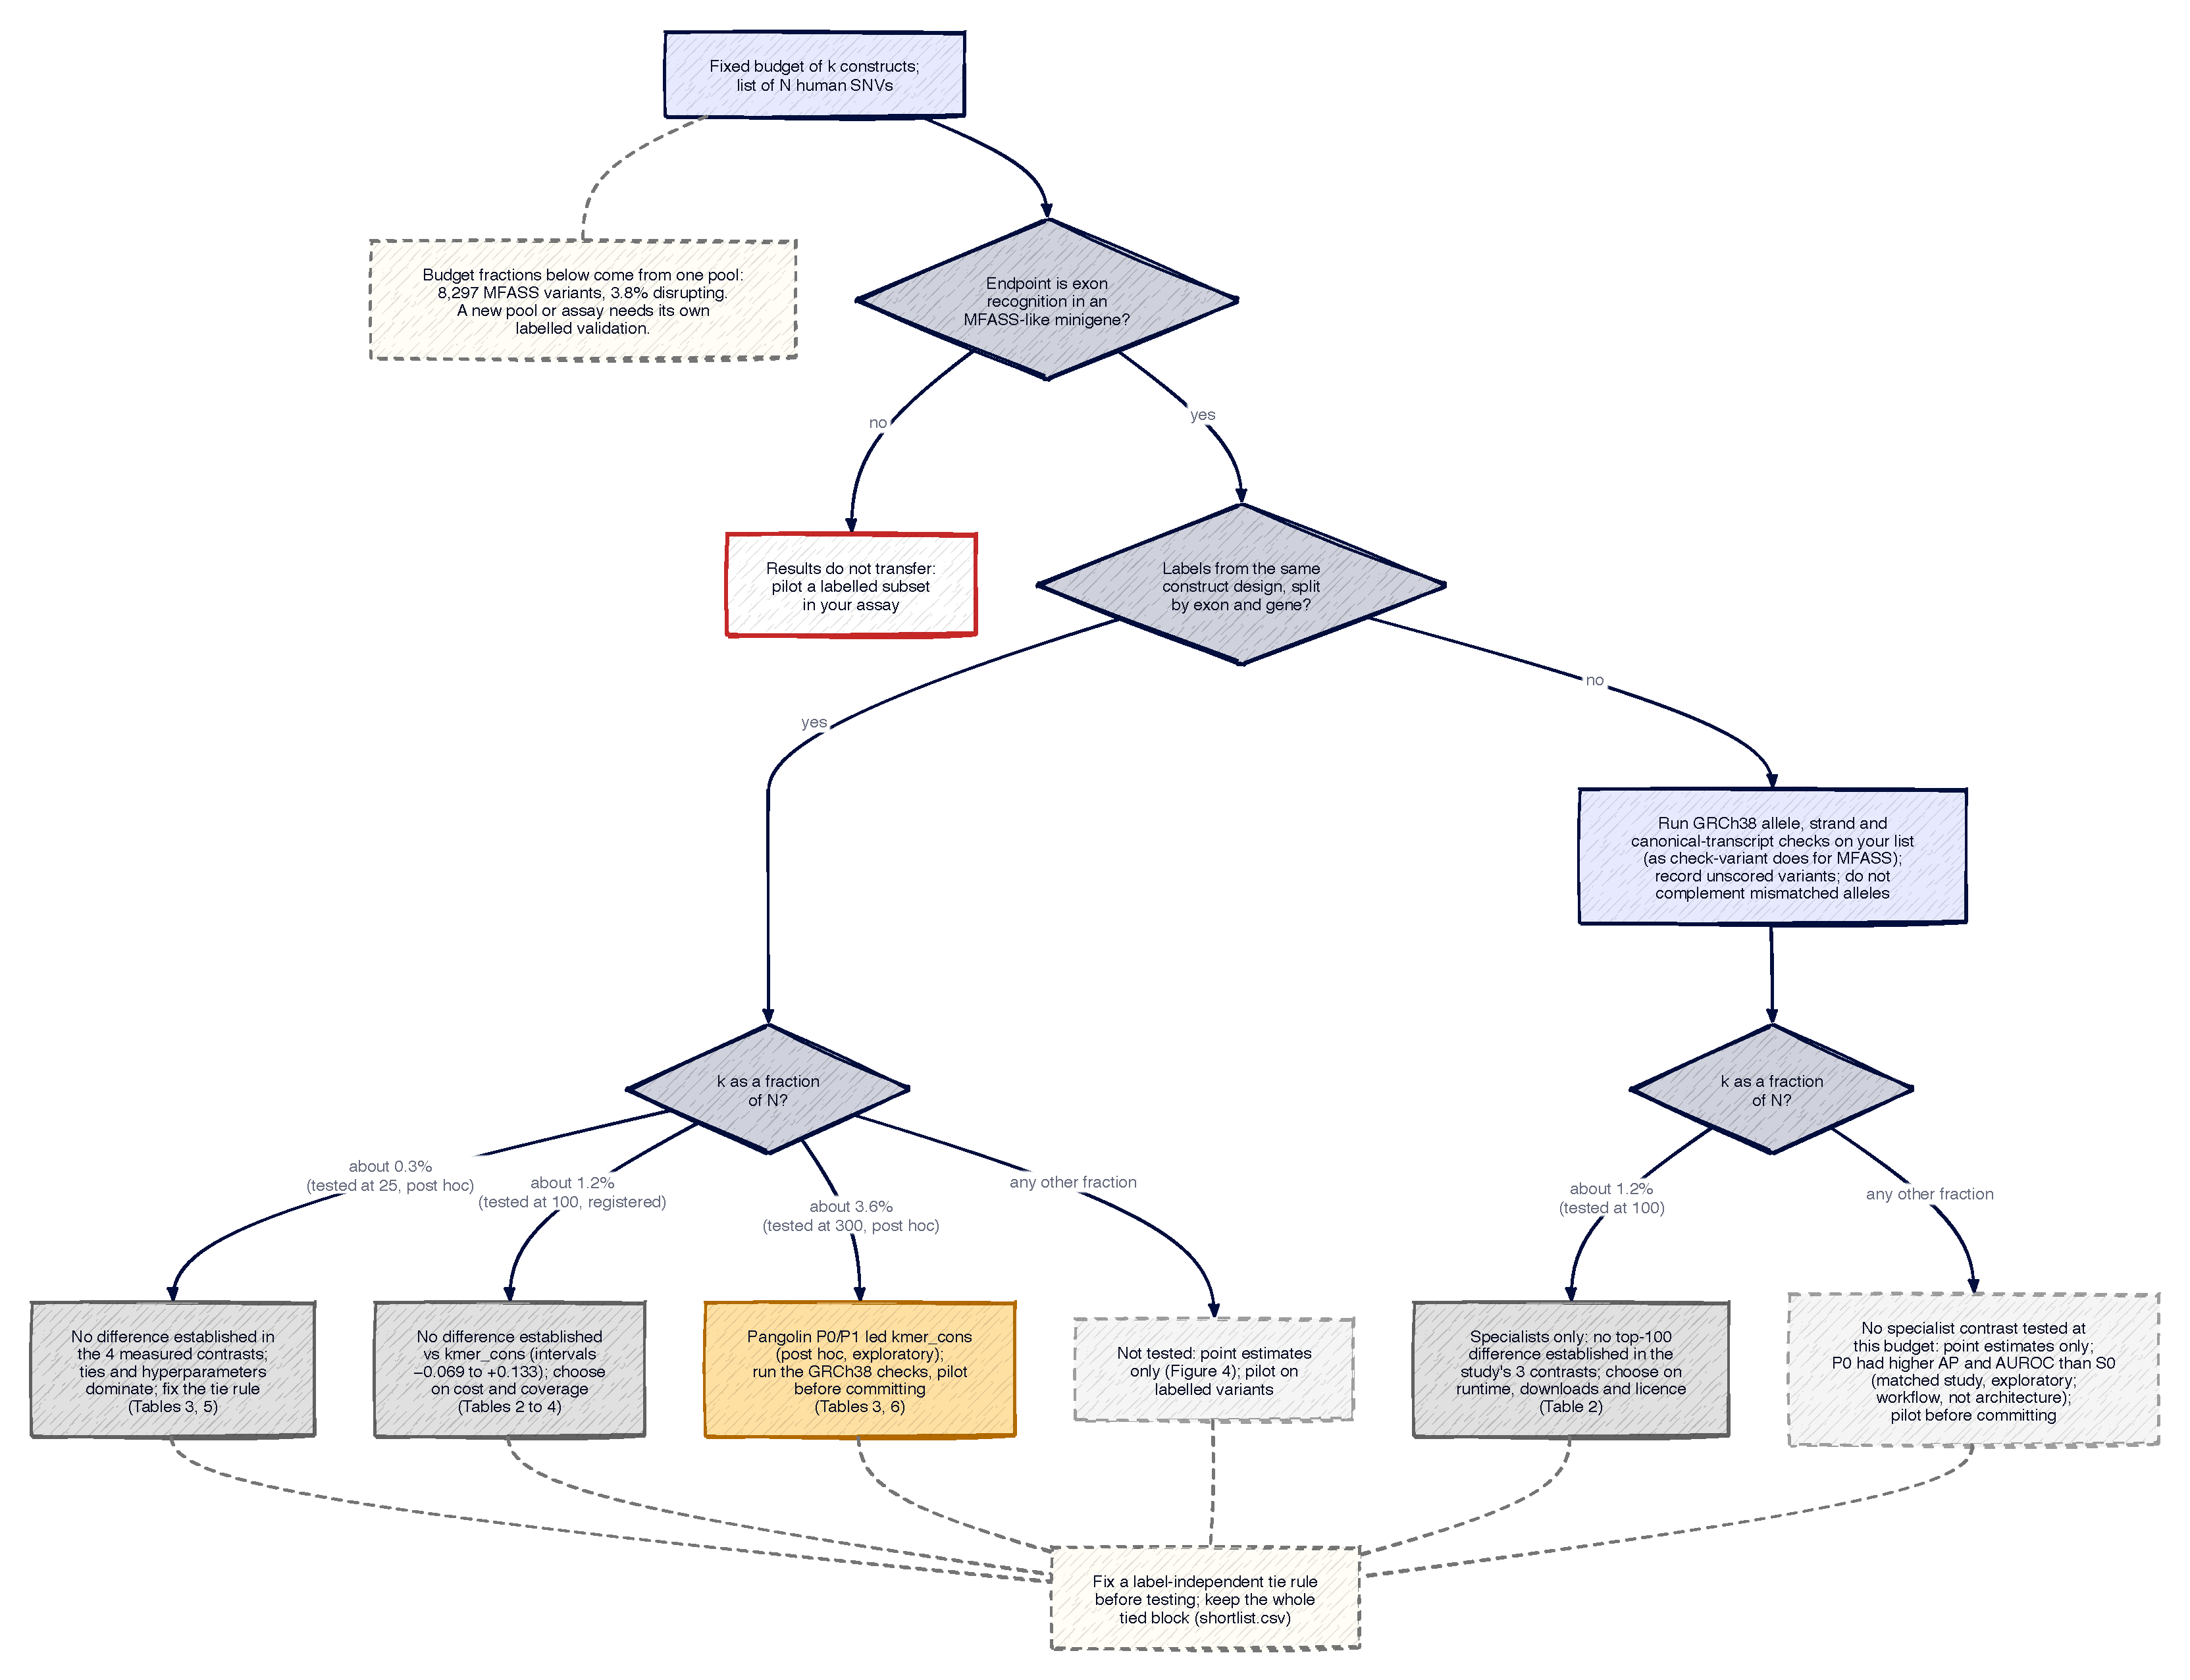
\includegraphics[width=\linewidth,height=0.76\textheight,keepaspectratio]{06-selection-flowchart.pdf}
\caption{\textbf{Selection flowchart} (original Figure~6, converted from
\texttt{article/\allowbreak assets/\allowbreak 06-selection-flowchart.svg}; D2 source
\texttt{article/\allowbreak assets/\allowbreak 06-selection-flowchart.d2}). Questions: is the endpoint MFASS-like minigene
exon recognition; do same-design labels exist; what fraction of the list is the budget. Terminals cite the original
Tables~2--6 (here Tables~\ref{tab:b100}, \ref{tab:contrasts-hist}, \ref{tab:contrasts-sel}, \ref{tab:budgets} and
\ref{tab:bands}); untested fractions end at ``not tested'', not at a recommendation. The vector figure can be zoomed;
Table~\ref{tab:glance} gives the same routes in readable form.}
\label{fig:flow}
\end{center}
\end{landscape}
\restoregeometry

\section{Provenance, supplement and evidence mapping}\label{app:provenance}
\paragraph{Supplement S1 (original article).} The full original article, \emph{Choosing a Splicing Score for a Fixed
Minigene Budget: Baseline, SpliceAI and Pangolin on MFASS} (published 30 September 2026), is retained unchanged in the
repository as \texttt{article/published-original.md} (byte-identical to the published source) and is embedded in this
PDF as the attachment \texttt{S1-published-original.md}. The repository copy \texttt{article/original.md} differs only in
local links. The original contains a frequently-asked-questions block and the reader-facing narrative that this
manuscript restructures; every scientific result it reports appears in this manuscript, and the section-by-section
mapping is in \texttt{evidence/paper-migration/content-coverage.md}.

\paragraph{Evidence ledger.} \texttt{evidence/paper-migration/claims-ledger.json} links each substantive claim to the
historical artifact (archive member or article text), a pointer inside it and its SHA-256. The archived outputs
(\texttt{downloads/splice-shortlist-outputs.zip}) were read in memory without extraction; their member digests are in
\texttt{evidence/reference-output-members.json}. The table generator (\texttt{scripts/paper\_extract.py}) stops the build
if any generated value that also appears in the original article differs from it (evidence-map items T2--T6, C-POP,
C-OVERLAP, F4, M-STUDY); the recorded cross-check found no difference. Values that the original did not print are
formatted directly from the digest-checked archive members.

\paragraph{Citation note.} The companion README cites the MFASS paper as \emph{Mol Cell} 2018 (its online date); this
manuscript follows the original article's issue citation (2019;73(1):183--194.e8)~\citep{chong2019mfass}. Literature
claims were verified for the original article on 30 September 2026 and were not re-retrieved during migration.

\end{document}
